%%%%%%%%%%%%%%%%%%%%%%%%%%%%%%%%%%%%%%%%%%%%%%%%%%%%%%%%%%%%%%%%%%%%%%%%%%%%%%%%
%%%%%%%%%%%%%%%%%%%%%%%%%%%%%%%%%%%%%%%%%%%%%%%%%%%%%%%%%%%%%%%%%%%%%%%%%%%%%%%%
%%% Template for AIMS Rwanda Assignments         %%%              %%%
%%% Author:   AIMS Rwanda tutors                             %%%   ###        %%%
%%% Email: tutors2017-18@aims.ac.rw                               %%%   ###        %%%
%%% Copyright: This template was designed to be used for    %%% #######      %%%
%%% the assignments at AIMS Rwanda during the academic year %%%   ###        %%%
%%% 2017-2018.                                              %%%   #########  %%%
%%% You are free to alter any part of this document for     %%%   ###   ###  %%%
%%% yourself and for distribution.                          %%%   ###   ###  %%%
%%%                                                         %%%              %%%
%%%%%%%%%%%%%%%%%%%%%%%%%%%%%%%%%%%%%%%%%%%%%%%%%%%%%%%%%%%%%%%%%%%%%%%%%%%%%%%%
%%%%%%%%%%%%%%%%%%%%%%%%%%%%%%%%%%%%%%%%%%%%%%%%%%%%%%%%%%%%%%%%%%%%%%%%%%%%%%%%


%%%%%% Ensure that you do not write the questions before each of the solutions because it is not necessary. %%%%%% 

\documentclass[12pt,a4paper]{article}

%%%%%%%%%%%%%%%%%%%%%%%%% packages %%%%%%%%%%%%%%%%%%%%%%%%
\usepackage{amsmath}
\usepackage{amssymb}
\usepackage{amsthm}
\usepackage{amsfonts}
\usepackage{graphicx}
\usepackage[all]{xy}
\usepackage{tikz}
\usepackage{verbatim}
\usepackage[left=2cm,right=2cm,top=3cm,bottom=2.5cm]{geometry}
\usepackage{hyperref}
\usepackage{caption}
\usepackage{subcaption}
\usepackage{multirow}
\usepackage{psfrag}

%%%%%%%%%%%%%%%%%%%%% students data %%%%%%%%%%%%%%%%%%%%%%%%
\newcommand{\student}{Professor of \LaTeX}
\newcommand{\course}{Latex\_Catch\_up}
\newcommand{\assignment}{01}

%%%%%%%%%%%%%%%%%%% using theorem style %%%%%%%%%%%%%%%%%%%%
\newtheorem{thm}{Theorem}
\newtheorem{lem}[thm]{Lemma}
\newtheorem{defn}[thm]{Definition}
\newtheorem{exa}[thm]{Example}
\newtheorem{rem}[thm]{Remark}
\newtheorem{coro}[thm]{Corollary}
\newtheorem{quest}{Question}[section]

%%%%%%%%%%%%%%  Shortcut for usual set of numbers  %%%%%%%%%%%

\newcommand{\N}{\mathbb{N}}
\newcommand{\Z}{\mathbb{Z}}
\newcommand{\Q}{\mathbb{Q}}
\newcommand{\R}{\mathbb{R}}
\newcommand{\C}{\mathbb{C}}

%%%%%%%%%%%%%%%%%%%%%%%%%%%%%%%%%%%%%%%%%%%%%%%%%%%%%%%555
\begin{document}

%%%%%%%%%%%%%%%%%%%%%%% title page %%%%%%%%%%%%%%%%%%%%%%%%%%
\thispagestyle{empty}
\begin{center}
\textbf{AFRICAN INSTITUTE FOR MATHEMATICAL SCIENCES \\[0.5cm]
(AIMS RWANDA, KIGALI)}
\vspace{1.0cm}
\end{center}

%%%%%%%%%%%%%%%%%%%%% assignment information %%%%%%%%%%%%%%%%
\noindent
\rule{17cm}{0.2cm}\\[0.3cm]
Name: \student \hfill Assignment Number: \assignment\\[0.1cm]
Course: \course \hfill Date: \today\\
\rule{17cm}{0.05cm}
\vspace{1.0cm}

\section{Theoretical exercice}

Everyone have to type this document as it is.

\begin{thm}
Let n and m be integers. Then
\begin{itemize}
	\item [i.] if $n$ and $m$ are both even, then $n + m$ is even,
	
	\item [ii.] if $n$ and m are both odd, then $n + m$ is even,
	
	\item [iii.] if one of $n$ and $m$ is even and the other is odd, then $n + m$ is odd.
\end{itemize}

\end{thm}

\begin{proof}
	
 \begin{itemize}
 	\item [i.]  If $n$ and $m$ are even, then there exist integers $k$ and $j$ such that $n = 2k$ and $m = 2j$. Then
 	\begin{align*}
 		n + m &= 2k + 2j\\
 		&= 2(k + j).
 	\end{align*}
 	
 	
 	And since $k, j \in \mathbb{Z} , (k + j) \in Z$. $\therefore$ $n$ + $m$ is even.
 	 
 \end{itemize}
 
\end{proof}

\begin{thm}
Let n $\in \mathbb{N}$, n $>$ 1. Suppose that n is not prime $\implies$ $2^{n}$-1 is not a prime.
\end{thm}

\begin{proof}
	Since n is \textbf{not} a prime, $\exists$ a,b $\in \mathbb{N}$ such that n = a $\times$ b, 1$<a,b<n$. Let x = $2^{b}-1$ and $y=1+2^{b}+2^{2b}+\dots+2^{(a-1)b}$. Then
	\begin{align*}
		xy&=(2^{b}-1)(1+2^{2b}+\dots+2^{(a-1)b})\\
		&=2^{b}+2^{2b}+2^{3b}+\dots+2^{ab}-1-2^{b}-2^{2b}-2^{3b}-\dots-2^{(a-1)b}\\
		&=2^{ab}-1\\
		&=2^{n}-1
	\end{align*}
Now notice that since $1< b < n$, we have that $1 < 2^{b} - 1$, so $1 < x < 2^{n}-1$.\\
Therefore, x is a positive factor, hence $2^{n}$-1 is \textbf{not} prime number.
\end{proof}
\newpage
\section{Sub-questions}
\begin{enumerate}
	\item
\begin{enumerate}
	\item Maxwell’s equations:
	\begin{subequations}\label{eq:group}
		\begin{align}
		  B'&=\nabla \times E\label{eq:A}\\
		  E'&=\nabla \times B-4 \pi j,\label{eq:B}
		\end{align}
	\item To show usage of L’Hôpital’s rule:
	\begin{align*}
	\lim\limits_{x \rightarrow 0} \frac{e^{x}-1}{2x} \frac{\left[\frac{0}{0}\right]}{H}\lim\limits_{x \rightarrow 0}\frac{e^{x}}{2}=\frac{1}{2}\\
	\iota_\tau(\vec{\lambda})= \sum_{(x,s)\in\tau} \log P (s \mid x) - \sum_{i=1}^{m} \frac{\lambda_{i}^{2}}{2\sigma^{2}}
	\end{align*}
	\item Complex numbers
	\begin{align*}
		z=\overbrace{\underbrace{x}_{real}+i+\underbrace{y}_{imaginary}}^{complex\ number}
	\end{align*}Mamy Rajaonarivelo
	\item To use brackets instead of braces use $\underbrace{}$ and $\overbrace{} commands$\\
	\begin{align*}
		y=a+f(\underbrace{bx}_{\geq 0 \ by \ assumption})=a+f(\underbrace{bx}_{\geq 0 \ by \ assumption})
	\end{align*}	
	\end{subequations}
\end{enumerate}	
\item 
\begin{enumerate}
	\item Using aligned braces for piecewise functions
	\begin{align*}
		f(x)=\begin{cases}
		x^{2} & \text{:$x<0$}\\
		                 x^{3}&\text{:$x\geq 0$}\end{cases}
	\end{align*}
	\item The cases environment allows the writing of piecewise functions
	\begin{align*}
		u(x)=\begin{cases}
		\exp x & \text{if $x\geq 0$}\\
		1 &\text{if $x < 0$}\end{cases}
	\end{align*}
	\item Matrix and array
	\begin{align*}
	&\begin{matrix}
	a & b & c\\
	d & e & f\\
	g & h & i
	\end{matrix}
	\end{align*}
	
	\begin{align*}	
	A_{m,n} = 
	&\begin{pmatrix}
	a_{1,1} & a_{1,2} & \cdots & a_{1,n} \\
	a_{2,1} & a_{2,2} & \cdots & a_{2,n} \\
	\vdots  & \vdots  & \ddots & \vdots  \\
	a_{m,1} & a_{m,2} & \cdots & a_{m,n} 
	\end{pmatrix}
	\end{align*}
	\begin{align*}
	M=
		\begin{bmatrix}
		\frac{5}{6} & \frac{1}{6} & 0\\
		\frac{5}{6} & 0 & \frac{1}{6}\\
		0 & \frac{5}{6} & \frac{1}{6}
		\end{bmatrix}
	\end{align*}
	\begin{align*}
	M = \bordermatrix{~ & x & y \cr
		A & 1 & 0 \cr
		B & 0 & 1 \cr}
	\end{align*}
	\item Equation columns\\
	\begin{align*}
		&f(x)=ax^{2}+bx+c & &g(x)=dx^{3}\\
		&f'(x)=2ax+b & &g'(x)=3dx^{2}
	\end{align*}
	\item If you want a brace to continue across a new line, do the following:\\
	\begin{align}
	f(x) &= x^4 + 7x^3 + 2x^2 \nonumber \\
	&\qquad {} + 10x + 12
	\end{align}
	\item
	\begin{equation}
	\boxed{x^2+y^2 = z^2}
	\end{equation}	
\item
	\begin{equation}
	\prod_{\substack{
			1\le i \le n\\
			1\le j \le m}}
	M_{i,j}
	\end{equation}
	\item
	\begin{equation}
	x = a_0 + \frac{1}{a_1 + \frac{1}{a_2 + \frac{1}{a_3 + a_4}}}
	\end{equation}

\item 
\begin{align*}
	cos(2\theta)=cos^{2}\theta-sin^{2}\theta
\end{align*}
\begin{align*}
	\frac{n!}{k!(n-k)!} = \binom{n}{k}
\end{align*}
\begin{align*}
	\frac{\frac{1}{x}+\frac{1}{y}}{y-z}
\end{align*}
\begin{equation}
\frac{
	\begin{array}[b]{r}
	\left( x_1 x_2 \right)\\
	\times \left( x'_1 x'_2 \right)
	\end{array}
}{
	\left( y_1y_2y_3y_4 \right)
}
\end{equation}
\item 
\begin{align*}
&\vdots\\ 
&=12+7 \int_0^2
\left(
-\frac{1}{4}\left(e^{-4t_1}+e^{4t_1-8}\right)
\right)\,dt_1\displaybreak[3]\\
&= 12-\frac{7}{4}\int_0^2 \left( e^{-4t_1}+e^{4t_1-8} \right)\,dt_1\\
&\vdots % 
\end{align*}

\item Differential equations\\
\begin{align*}
\frac{\partial u}{\partial t}
	= h^2 \left( \frac{\partial^2 u}{\partial x^2}
	+ \frac{\partial^2 u}{\partial y^2}
	+ \frac{\partial^2 u}{\partial z^2} \right) \
\end{align*}

\begin{table}[ht]
	
	\centering
	\caption{My caption}
	\label{tab:my_label}
	\begin{tabular}{ |p{2cm}|p{3cm}|p{3cm}| }%{|c|c|c|}
		\hline
		Name & \multicolumn{2}{|c|}{Bob}\\
		\hline
		Type & \multicolumn{2}{|c|}{Client} \\
		\hline
		\multirow{1}{*}{Parameters}&Param1 & Value\\ 
		\cline{2-3} 
		&Param2 &Value\\
		\cline{2-3}
		& Param3 &Value\\
		\hline
	\end{tabular}

\end{table}

\end{enumerate}
\end{enumerate}

\section{Equations}
The general form of a quadratic equation is given by\\
\begin{center}
	$ax^2 + bx +c = 0$,
\end{center}
where $a$, $b$ and $c$ are real numbers, and $a \neq0$.\\
If I want to number the equation, it will look like this\\
\begin{equation}
\label{eq:1}
ax^{2} + bx +c = 0,
\end{equation}

where $a$, $b$ and $c$ are real numbers, and $a \neq0$. Equation\ref{eq:1} is the general form of a quadratic equation. Below is a system of equations\\
\begin{equation}
\label{eq:2}
\int_{a}^{b} f(x) \,dx \ = (b-a)[\frac{f(a)+f(b)}{2}]
\end{equation}

\begin{equation}
\label{eq:3}
\int_{a}^{b} f(x) \,dx  = \frac{h}{2}\sum_{k=1}^{N}(f(x_k+1)+f(x_k)) 
\end{equation}

Equation\ref{eq:3} is the general form of equation \ref{eq:2}, where the limit of integration is partitioned into $N$ strips of equal intervals given by $h$.

\section{Tables}
\section{Figures}
\subsection{One figure}
Figure \ref{fig:trapez1.png} has only one picture. For pictures appearing side by side see section 5.2.
\subsection{Figures side by side}
This is how you put two pictures side by side. Note that each subfigure has its own caption, and the entire figure has a caption which gives a more general description of the figures. Figure \ref{fig:1} is the same as figure \ref{fig:trapez1.png}. They both correspond to equation \ref{eq:2}. Figure \ref{fig:2} corresponds to equation \ref{eq:3}. Figure \ref{fig:3} is a pictorial description of equations \ref{eq:2}, and \ref{eq:3}.\\

\begin{figure}[h]
	\centering
	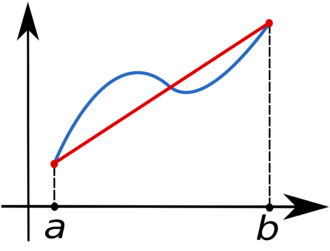
\includegraphics[scale=0.7]{trapez1.png}
	\caption{The simplest form of the trapezoidal rule.}
	\label{fig:trapez1.png}
\end{figure}

\begin{figure}[h]
	\begin{subfigure}[b]{0.45\textwidth}
		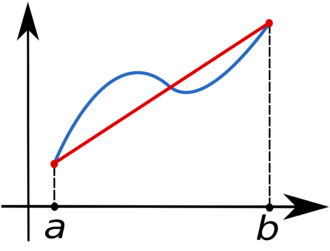
\includegraphics[width=\textwidth]{trapez1.png}
		\caption{Trapezoidal rule with a single strip.}
		\label{fig:1}
	\end{subfigure}
	\begin{subfigure}[b]{0.45\textwidth}
		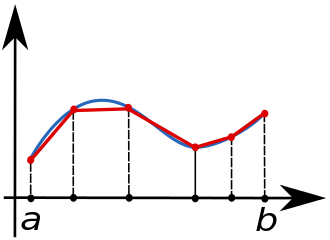
\includegraphics[width=\textwidth]{trapez2.png} 
		\caption{Trapezoidal rule with N equally spaced strips.}
		\label{fig:2}
	\end{subfigure}
	\caption{Trapezoidal rules}
	\label{fig:3}
\end{figure}

\newpage
\subsection{Examples: How to cite}
To cite a reference, you use  $\setminus$cite$\{$key$\}$. For example: For a compiled reading history see \cite{notes}. To know more about Western learning in mordern Japan, we recommend \cite{fo, notes}. There is a comprehensive write up in \cite{norman} about the emergence of Japan as a modern state.

\newpage
\begin{thebibliography}{99}
	
	\bibitem{notes} John W. Dower {\em Readings compiled for History
		21.479.}  1991.
	
	\bibitem{norman} E. H. Norman {\em Japan's emergence as a modern
		state} 1940: International Secretariat, Institute of Pacific
	Relations.
	
	\bibitem{fo} Bob Tadashi Wakabayashi {\em Anti-Foreignism and Western Learning in Early-Modern Japan} 1986: Harvard University Press.
\end{thebibliography}

\end{document}